% First-Mover Bias in Gradient Boosting Explanations:
% Mechanism, Detection, and Resolution
%
% Caraker, Arnold, Rhoads (2026)
%
\documentclass[11pt]{article}

% --- Packages ---
\usepackage[margin=1in]{geometry}
\usepackage{amsmath,amssymb,amsfonts}
\usepackage{graphicx}
\usepackage{booktabs}
\usepackage{multirow}
\usepackage{xcolor}
\usepackage{natbib}
\usepackage{algorithm}
\usepackage{algorithmic}
\usepackage{caption}
\usepackage{subcaption}
\usepackage{tikz}
\usetikzlibrary{arrows.meta,positioning,shapes.geometric,fit}
\usepackage{hyperref}

\hypersetup{colorlinks=true, linkcolor=blue, citecolor=blue, urlcolor=blue}

% --- Graphics path ---
\graphicspath{{../results/figures/}{../notebooks/results/figures/}}

% --- Macros ---
\newcommand{\dash}{\textsc{DASH}}
\newcommand{\rhovar}{\rho}
\newcommand{\eg}{e.g.,\ }
\newcommand{\ie}{i.e.,\ }
\newcommand{\wrt}{w.r.t.\ }

\title{%
  \textbf{First-Mover Bias in Gradient Boosting Explanations:} \\[6pt]
  \large Mechanism, Detection, and Resolution
}

\author{
  Drake Caraker\thanks{Corresponding author.} \qquad
  Bryan Arnold \qquad
  David Rhoads \\[4pt]
  \textit{Independent Researchers} \\
  \texttt{puremath86@gmail.com} (Caraker \& Arnold) \quad \texttt{drhoads9@gmail.com} (Rhoads)
}

\date{March 2026}

\begin{document}
\maketitle

% ===========================================================================
\begin{abstract}
We identify \emph{first-mover bias}---a path-dependent concentration of
feature importance caused by sequential residual fitting in gradient
boosting---as a specific mechanistic cause of the well-known instability of
SHAP-based feature rankings under multicollinearity. When correlated features
compete for early splits, gradient boosting creates a self-reinforcing
advantage for whichever feature is selected first: subsequent trees inherit
modified residuals that favor the incumbent, concentrating SHAP importance on
an arbitrary feature rather than distributing it across the correlated group.
Scaling up a single model amplifies this effect---a Large Single Model with
the same compute budget as our method produces the \emph{worst} explanations
of any approach tested.

We demonstrate that \emph{model independence} is sufficient to resolve
first-mover bias. Both our proposed method, \dash{} (Diversified Aggregation
of SHAP), and simple seed-averaging (Stochastic Retrain) restore stability
by breaking the sequential dependency chain, confirming that the operative
mechanism is independence between explained models, not any particular
aggregation strategy. At $\rhovar = 0.9$, both methods achieve stability
$\approx 0.977$ (not significantly different), while the standard
single-best workflow degrades to $0.958$ and the Large Single Model to
$0.938$. On the Breast Cancer dataset, \dash{} improves stability from
$0.32$ to $0.93$ ($+0.61$), comparing against a compute-matched
Single Best baseline ($M{=}200$).

\dash{} additionally provides two novel diagnostic tools---the Feature
Stability Index (FSI) and Importance-Stability (IS) Plot---that detect
first-mover bias without ground truth, enabling practitioners to audit
explanation reliability before acting on feature rankings. Software and
reproducible benchmarks are available at
\url{https://github.com/DrakeCaraker/dash-shap}.
\end{abstract}

\textbf{Keywords:} first-mover bias, SHAP, feature importance, multicollinearity,
model independence, gradient boosting, explainability, Rashomon effect

% ===========================================================================
\section{Introduction}
\label{sec:introduction}

The standard workflow for explaining gradient-boosted tree predictions is
deceptively simple: train a model, compute SHAP values, report the feature
importance ranking. This ranking drives consequential decisions across
science, industry, and regulation---it selects features for production
pipelines, generates hypotheses in biomedical research, and satisfies
regulatory auditors reviewing algorithmic systems. The workflow is
ubiquitous and is treated as reliable.

It is not. When features are correlated, SHAP-based importance rankings
become unstable. At each split, a gradient-boosted tree must choose one
feature from a correlated set. Since correlated features carry nearly
identical predictive signal, the choice is governed by marginal numerical
differences---effectively arbitrary. The model's predictions are robust to
this choice, but the SHAP values are not: changing the random seed, the
learning rate, or the tree depth can swap the positions of correlated
features in the importance ranking without meaningfully altering predictive
accuracy. This is a manifestation of the Rashomon effect
\citep{breiman2001statistical} applied to explanations rather than
predictions.

The problem is pervasive because multicollinearity is pervasive. In
clinical datasets, radius, perimeter, and area measure the same underlying
tumor geometry. In materials science, atomic-level properties of
constituent elements are correlated by construction. In economics and
social science, income, education, and occupation form tightly coupled
clusters. Any dataset where features were not specifically decorrelated
before modeling is susceptible.

\paragraph{Why bigger models make it worse.}
The intuitive response to unstable explanations is to train a more powerful
model. We demonstrate that this is counterproductive. A single large
XGBoost model with thousands of trees and the same total tree count as \dash{} ($M \times \sim$75 $\approx$ 15\,000 trees) produces the \emph{worst} explanations of any method
tested---worse on stability, accuracy, and equity simultaneously. The
mechanism is \emph{sequential residual dependency}: in gradient boosting,
each tree fits the residuals of all previous trees. If tree~1 selects
feature~$A$ from a correlated pair $(A, B)$, it partially removes $A$'s
signal from the residuals. Subsequent trees find both $A$ and $B$ less
useful, but $A$ slightly more so because the residual structure favors the
feature that was partially captured. Over thousands of iterations, this
creates a ``first-mover advantage'' that concentrates importance on
whichever feature happened to be selected first---an artifact of
optimization path dependence, not a property of the data.

\paragraph{Our contribution.}
We propose \dash{} (Diversified Aggregation of SHAP), a five-stage
pipeline that produces stable, accurate, and equitable feature importance
explanations. The key insight is that explanation instability is a property
of individual models, not of the data: training enough diverse models and
averaging their SHAP values causes the arbitrary choices to cancel,
revealing the true underlying importance structure. Specifically, \dash{}:

\begin{enumerate}
  \item Trains a population ($M = 200$) of XGBoost models with
    randomly sampled hyperparameters, including deliberately low
    \texttt{colsample\_bytree} (0.1--0.5) to force feature diversity.
  \item Filters for predictive quality, retaining only models within
    $\varepsilon$ of the best validation score.
  \item Selects a diverse subset ($K \leq 30$) via greedy max-min
    dissimilarity on feature utilization vectors.
  \item Computes interventional TreeSHAP for each selected model and
    averages the SHAP matrices element-wise.
  \item Provides diagnostic tools (Feature Stability Index, IS Plot,
    local disagreement maps) for auditing explanation reliability.
\end{enumerate}

We make four contributions:
\begin{itemize}
  \item \textbf{Phenomenon.} Feature selection bias in ensemble methods
    is well known \citep{strobl2007bias, hooker2019please}; we identify
    the specific mechanistic pathway---sequential residual dependency
    in gradient boosting---through which it concentrates SHAP-based
    feature attributions on arbitrary features under collinearity.
  \item \textbf{Principle.} We demonstrate that model independence is
    sufficient to resolve first-mover bias.
    Both \dash{} (deliberate diversity) and Stochastic Retrain (seed
    diversity) restore stability to the same level, confirming that
    the operative mechanism is independence rather than any particular
    aggregation strategy.
  \item \textbf{Diagnostics.} The Feature Stability Index (FSI) and
    Importance-Stability (IS) Plot detect first-mover bias without
    access to ground truth, enabling practitioners to audit explanation
    reliability.
  \item \textbf{Method.} \dash{} (Diversified Aggregation of SHAP) is
    an engineered pipeline that operationalizes the independence principle
    with forced feature restriction, diversity-aware model selection,
    and integrated diagnostics.
\end{itemize}


% ===========================================================================
\section{Related Work}
\label{sec:related}

\paragraph{SHAP and model explanations.}
SHAP values \citep{lundberg2017unified} provide a theoretically grounded
decomposition of predictions into feature contributions, drawing on the
Shapley value framework from cooperative game theory
\citep{shapley1953value}. TreeSHAP \citep{lundberg2020local} enables
efficient exact computation for tree-based models. While SHAP satisfies
desirable axiomatic properties (local accuracy, missingness, consistency),
these guarantees are conditioned on a fixed model. When the model changes---
even slightly---the SHAP values can change substantially.

\paragraph{Instability of feature importance.}
The instability of SHAP values under model perturbation has been noted by
several authors. \citet{fisher2019all} formalize the Rashomon set---the
collection of models with near-optimal performance---and show that
variable importance can vary widely across this set.
\citet{marx2023but} demonstrate that SHAP-based feature attributions
are sensitive to reference distribution choices.
The problem is especially acute for correlated features, where SHAP must
distribute credit among features that carry overlapping information
\citep{kumar2020problems, chen2020true}.

\paragraph{Ensemble explanations.}
\citet{paillard2025ensemble} argue for computing SHAP values from a single
large ensemble rather than aggregating explanations from multiple models,
on the grounds that a single ensemble provides a consistent explanation.
Our results challenge this recommendation: the single-ensemble approach
(our ``Ensemble SHAP'' baseline) does not resolve the instability caused
by correlated features and, when taken to its extreme (the Large Single
Model), amplifies it.

\paragraph{Stable explanations.}
\citet{alvarez2018towards} propose metrics for explanation stability.
\citet{krishna2022disagreement} study disagreement among different
explanation methods applied to the same model. Our work addresses a
different source of disagreement: the same explanation method (SHAP)
applied to different-but-equally-valid models.

\paragraph{Feature selection under multicollinearity.}
Classical approaches to multicollinearity include variance inflation
factors \citep{obrien2007caution}, principal component regression, and
elastic net regularization \citep{zou2005regularization}. Stability
selection \citep{meinshausen2010stability} addresses a related problem
by subsampling data and tracking which features are consistently
selected across subsamples. Permutation importance
\citep{altmann2010permutation} offers an alternative to SHAP with
different stability properties. Causal Shapley values
\citep{heskes2020causal} provide principled handling of correlated
features through causal structure. These methods operate at the
model-fitting or feature-selection stage. \dash{} operates at the
explanation stage, preserving the original feature space while
stabilizing the attributions.


% ===========================================================================
\section{Problem Formulation}
\label{sec:problem}

\subsection{Setup}

Let $\mathbf{X} \in \mathbb{R}^{N \times P}$ be a dataset of $N$
observations and $P$ features, with target $\mathbf{y} \in \mathbb{R}^N$.
Let $f_\theta$ denote a gradient-boosted tree model trained with
hyperparameters $\theta$. Let $\phi_j^{(i)}(f_\theta)$ denote the SHAP
value of feature $j$ for observation $i$ under model $f_\theta$.

The \emph{global feature importance} vector is
\begin{equation}
  \bar{I}_j(f_\theta) = \frac{1}{N'} \sum_{i=1}^{N'} |\phi_j^{(i)}(f_\theta)|,
  \label{eq:global_importance}
\end{equation}
where $N'$ is the number of reference observations.

\subsection{The instability problem}

Consider two models $f_{\theta_1}$ and $f_{\theta_2}$, both trained on the
same data with different hyperparameters $\theta_1 \neq \theta_2$, such
that their predictive performance is comparable:
$|\text{RMSE}(f_{\theta_1}) - \text{RMSE}(f_{\theta_2})| < \varepsilon$.
Despite this, the importance rankings
$\text{rank}(\bar{I}(f_{\theta_1}))$ and
$\text{rank}(\bar{I}(f_{\theta_2}))$ can differ substantially when
features are correlated.

Formally, let $\mathcal{G} = \{G_1, \ldots, G_L\}$ be a partition of
$\{1, \ldots, P\}$ into groups of correlated features, where features
within group $G_l$ have pairwise correlation $\geq \rhovar$. A single
model $f_\theta$ produces importance $\bar{I}_j$ that is concentrated on
an arbitrary subset of each group---typically the feature(s) selected at
early splits. This concentration is unstable: different $\theta$ values
produce different concentrations within the same group.

\subsection{Sequential residual dependency}

In gradient boosting, model $f$ is constructed as $f =
\sum_{t=1}^{T} h_t$, where tree $h_t$ is fit to the residuals
$r_t = y - \sum_{s<t} h_s(x)$. If tree $h_1$ splits on feature $j \in
G_l$, it partially removes $j$'s signal from $r_2$. Since feature $k
\in G_l$ ($k \neq j$) carries overlapping signal, $k$'s marginal gain
for $r_2$ is also reduced---but $j$ retains a slight residual advantage
from its own partial fit. Over $T$ iterations, this creates a
path-dependent concentration of splits on the first-selected feature
within each correlated group. We coin the term \emph{sequential residual
dependency} to describe this mechanism, which is related to the
well-known feature selection bias in boosted ensembles but specifically
concerns its effect on post-hoc feature attributions.

\subsection{Desiderata}

A good feature importance method under multicollinearity should satisfy:
\begin{enumerate}
  \item \textbf{Stability}: Repeated runs with different random seeds or
    hyperparameters should produce consistent rankings.
  \item \textbf{Accuracy}: The ranking should correlate with the true
    data-generating process when ground truth is available.
  \item \textbf{Equity}: Correlated features contributing equally to the
    target should receive similar importance.
  \item \textbf{Safety}: The method should not degrade explanations or
    predictions when features are uncorrelated.
\end{enumerate}


% ===========================================================================
\section{Method: DASH}
\label{sec:method}

\dash{} is a five-stage pipeline (Figure~\ref{fig:pipeline}):

\begin{figure}[h]
\centering
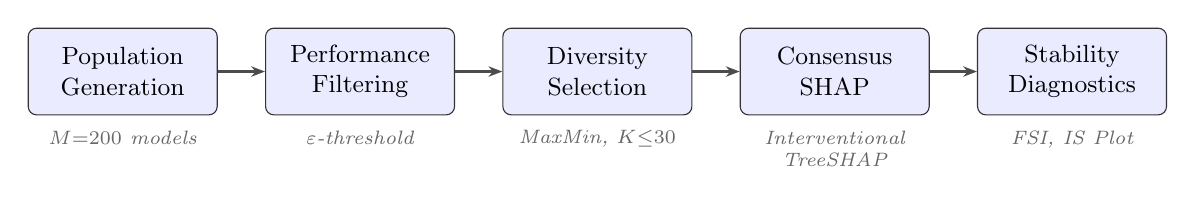
\begin{tikzpicture}[
  stage/.style={rectangle, draw=black!80, fill=blue!8, rounded corners=3pt,
    minimum height=1.1cm, minimum width=2.4cm, align=center, font=\small},
  arr/.style={-{Stealth[length=5pt]}, thick, color=black!70},
  note/.style={font=\scriptsize\itshape, color=black!60, align=center},
]
  \node[stage] (pop)  {Population\\Generation};
  \node[stage, right=0.6cm of pop]  (filt) {Performance\\Filtering};
  \node[stage, right=0.6cm of filt] (div)  {Diversity\\Selection};
  \node[stage, right=0.6cm of div]  (cons) {Consensus\\SHAP};
  \node[stage, right=0.6cm of cons] (diag) {Stability\\Diagnostics};

  \draw[arr] (pop)  -- (filt);
  \draw[arr] (filt) -- (div);
  \draw[arr] (div)  -- (cons);
  \draw[arr] (cons) -- (diag);

  \node[note, below=2pt of pop]  {$M{=}200$ models};
  \node[note, below=2pt of filt] {$\varepsilon$-threshold};
  \node[note, below=2pt of div]  {MaxMin, $K{\leq}30$};
  \node[note, below=2pt of cons] {Interventional\\TreeSHAP};
  \node[note, below=2pt of diag] {FSI, IS~Plot};
\end{tikzpicture}
\caption{The \dash{} five-stage pipeline. Models are trained independently
(Stage~1), filtered for quality (Stage~2), selected for diversity (Stage~3),
explained via TreeSHAP and averaged (Stage~4), and audited for stability
(Stage~5).}
\label{fig:pipeline}
\end{figure}

\subsection{Stage 1: Population Generation}

We train $M$ XGBoost models with hyperparameters randomly sampled from a
search space $\Theta$ (Table~\ref{tab:search_space}). The critical
parameter is \texttt{colsample\_bytree}, sampled from
$\{0.1, 0.15, 0.2, 0.25, 0.3, 0.4, 0.5\}$, which restricts each tree
to a random subset of features. This forces different models to rely on
different members of correlated groups. Each model is trained independently
with early stopping, using a separate random seed to diversify initialization.

\begin{table}[h]
\centering
\caption{Hyperparameter search space for population generation.}
\label{tab:search_space}
\begin{tabular}{ll}
\toprule
\textbf{Parameter} & \textbf{Values} \\
\midrule
\texttt{max\_depth}         & $\{3, 4, 5, 6, 8, 10, 12\}$ \\
\texttt{learning\_rate}     & $\{0.01, 0.03, 0.05, 0.1, 0.2, 0.3\}$ \\
\texttt{colsample\_bytree}  & $\{0.1, 0.15, 0.2, 0.25, 0.3, 0.4, 0.5\}$ \\
\texttt{subsample}          & $\{0.5, 0.6, 0.7, 0.8, 0.9, 1.0\}$ \\
\texttt{reg\_alpha}         & $\{0, 0.01, 0.1, 1.0, 5.0, 10.0\}$ \\
\texttt{reg\_lambda}        & $\{0, 0.01, 0.1, 1.0, 5.0, 10.0\}$ \\
\texttt{min\_child\_weight} & $\{1, 3, 5, 10, 20\}$ \\
\bottomrule
\end{tabular}
\end{table}

\subsection{Stage 2: Performance Filtering}

We retain models whose validation score is within $\varepsilon$ of the
best:
\begin{equation}
  \mathcal{F} = \{i : |s_i - s^*| \leq \varepsilon\},
  \quad s^* = \max_i s_i,
  \label{eq:filter}
\end{equation}
where $s_i$ is the negative RMSE (for regression) or AUC (for
classification) of model $i$. This ensures that all explanations come from
models that have learned meaningful signal. We use $\varepsilon = 0.08$
(absolute mode) for synthetic data and $\varepsilon = 0.05$ (relative
mode, retaining models within 5\% of the best score) for real-world
datasets.

\subsection{Stage 3: Diversity Selection}

From the filtered set $\mathcal{F}$, we select $K \leq K_{\max}$
models to maximize feature utilization diversity. We compute a
preliminary importance vector $\mathbf{v}_i$ for each model $i \in
\mathcal{F}$ using XGBoost's gain-based importance (faster than SHAP,
sufficient for measuring feature utilization patterns).

\paragraph{MaxMin selection (default).}
We use greedy max-min dissimilarity selection:
\begin{enumerate}
  \item Initialize with the highest-performing model.
  \item At each step, add the candidate $c$ that maximizes
    $\min_{s \in \mathcal{S}} d(c, s)$, where
    $d(c, s) = 1 - \hat{\mathbf{v}}_c \cdot \hat{\mathbf{v}}_s$
    and $\hat{\mathbf{v}}$ denotes $L_2$-normalized importance vectors.
  \item Stop when $K_{\max}$ is reached or the minimum distance falls
    below threshold $\delta$.
\end{enumerate}

This ensures each selected model is maximally different from all previously
selected models in its feature utilization pattern, without requiring
knowledge of the feature correlation structure.

\paragraph{Alternative: Deduplication selection.}
A simpler variant removes near-duplicate models (pairwise Spearman
$\rhovar > 0.95$ on importance vectors), retaining the better-performing
model from each pair. This provides a minimal-overhead diversity guarantee.

\subsection{Stage 4: Consensus SHAP}

We compute interventional TreeSHAP \citep{lundberg2020local} for each
selected model $i \in \mathcal{S}$ using a randomly sampled background
dataset of size $B = 100$. In our experiments, SHAP values are computed
on a held-out \emph{explain set} $X_{\text{explain}}$, which is disjoint
from the training set, the validation set used for performance filtering
(Stage~2), and the test set used for RMSE evaluation. This four-way split
(train/val/explain/test) prevents any overlap between the data used for
model selection, explanation computation, and predictive evaluation.
\begin{equation}
  \Phi^{(i)} \in \mathbb{R}^{N' \times P}, \quad i \in \mathcal{S}.
\end{equation}

The consensus SHAP matrix is the element-wise average:
\begin{equation}
  \bar{\Phi} = \frac{1}{|\mathcal{S}|} \sum_{i \in \mathcal{S}} \Phi^{(i)}.
  \label{eq:consensus}
\end{equation}

Because each model $i$ was trained independently, its arbitrary feature
selections within correlated groups are independent across models.
Averaging causes these arbitrary choices to cancel, distributing
importance proportionally across the group.

\subsection{Stage 5: Stability Diagnostics}

We introduce two diagnostic tools that quantify explanation reliability
without requiring ground-truth importance:

\paragraph{Feature Stability Index (FSI).}
For each feature $j$:
\begin{equation}
  \text{FSI}_j = \frac{\bar{\sigma}_j}{\bar{I}_j + \epsilon},
  \label{eq:fsi}
\end{equation}
where $\bar{\sigma}_j = \frac{1}{N'}\sum_i \text{std}_k[\phi_j^{(i)}(f_k)]$
is the mean (across observations) of the standard deviation (across models)
of SHAP values, and $\bar{I}_j$ is the consensus global importance
(Eq.~\ref{eq:global_importance}). High FSI indicates that a feature's
SHAP values vary substantially across models relative to its importance---
a signature of explanation instability, typically caused by collinearity.

\paragraph{Importance-Stability (IS) Plot.}
A scatter plot of $(\bar{I}_j, \text{FSI}_j)$ for each feature $j$,
partitioned into four quadrants by median thresholds:
\begin{itemize}
  \item \textbf{Quadrant I} (high importance, low FSI): \emph{Robust
    drivers}---features that are genuinely important and whose importance
    is stable across models.
  \item \textbf{Quadrant II} (high importance, high FSI): \emph{Collinear
    cluster members}---features that are important but whose specific
    attribution is unstable, indicating collinearity.
  \item \textbf{Quadrant III} (low importance, low FSI): \emph{Confirmed
    unimportant}---features that all models agree are unimportant.
  \item \textbf{Quadrant IV} (low importance, high FSI): \emph{Fragile
    interactions}---features with small but unreliable attributions.
\end{itemize}

The IS Plot functions as an unsupervised collinearity detector: features
in Quadrant~II are likely members of correlated groups, even without
computing the correlation matrix directly.


% ===========================================================================
\section{Experimental Design}
\label{sec:experiments}

\subsection{Synthetic data}

We generate data with $N = 5{,}000$ observations and $P = 50$ features
arranged in 10 groups of 5, with within-group correlation $\rhovar$.
The target follows a linear data-generating process (DGP):
\begin{equation}
  y = \sum_{g=1}^{10} \beta_g \cdot \bar{z}_g + \epsilon,
  \quad \epsilon \sim \mathcal{N}(0, 0.5^2),
\end{equation}
where $\bar{z}_g$ is the mean of features in group $g$ and
$\beta_g \in \{2.0, 1.5, 1.0, 0.8, 0.6, 0.4, 0.3, 0.2, 0.1, 0.0\}$.
By construction, the true importance of each feature within group $g$ is
defined as $|\beta_g|/5$ (uniform within group).

\paragraph{Caveat on ground-truth definition.}
This uniform definition presupposes equitable credit distribution
within correlated groups---precisely the property \dash{} is designed
to achieve. Alternative decompositions are valid: a single model that
correctly uses feature $A$ (not $B$) from a correlated pair has a
legitimate attribution where $A$ is important and $B$ is not. Our
accuracy metric therefore measures agreement with the equitable
decomposition, not ``correctness'' in an absolute sense. The accuracy
advantage of \dash{} should be interpreted as a consequence of its
equity properties rather than independent evidence of superiority.

For the nonlinear DGP, the target includes quadratic terms, interactions,
and a sinusoidal component:
\begin{equation}
  y = \beta_1 z_1^2 + \beta_2 z_1 z_2 + \beta_3 \sin(\pi z_3) +
  \sum_{g=4}^{10} \beta_g z_g + \epsilon.
\end{equation}

We sweep $\rhovar \in \{0.0, 0.5, 0.7, 0.9, 0.95\}$ with $N_{\text{reps}}
= 20$ repetitions at each level, regenerating data (same coefficients, new
random draws) for each repetition.

\subsection{Real-world datasets}

\paragraph{Breast Cancer Wisconsin.}
30 features derived from digitized images of fine-needle aspirates. Heavy
natural collinearity: 21 feature pairs have $|r| > 0.9$ (radius $\approx$
perimeter $\approx$ area). Binary classification task.

\paragraph{Superconductor.}
81 features describing physical and chemical properties of 21,263
superconducting materials. Regression task predicting critical temperature.
We use $\varepsilon = 0.05$ in relative mode (retaining models within
5\% of the best validation score).

\paragraph{California Housing.}
8 features describing housing characteristics of 20,640 California
census blocks. Regression task predicting median house value. Moderate
collinearity: several feature pairs with $|r| > 0.7$ (\eg income and
house value, latitude and longitude).
We use relative $\varepsilon = 0.05$ for scale-appropriate filtering.

\subsection{Methods compared}

We compare 9 methods (Table~\ref{tab:methods}):

\begin{table}[h]
\centering
\caption{Methods compared in the benchmark. All use XGBoost as the base learner.}
\label{tab:methods}
\begin{tabular}{llp{6.8cm}}
\toprule
& \textbf{Method} & \textbf{Description} \\
\midrule
\multirow{5}{*}{\rotatebox{90}{\scriptsize Dependent}}
  & Single Best       & Best of 30 hyperparameter-tuned models (standard practice) \\
  & Single Best ($M$) & Best of $M{=}200$ models (compute-matched to \dash{}) \\
  & Large Single Model & One XGBoost with $\sim$15K trees, low \texttt{colsample\_bytree} \\
  & LSM (Tuned)       & Grid search over \texttt{max\_depth}, \texttt{learning\_rate} \\
  & Ensemble SHAP     & Single 2000-tree ensemble (\texttt{colsample\_bytree}{=}0.8) \\
\midrule
\multirow{4}{*}{\rotatebox{90}{\scriptsize Independent}}
  & Stochastic Retrain & $K$ models, different seeds, same hyperparameters \\
  & Random Selection  & DASH population + filtering, random $K$ selection \\
  & Naive Top-$N$     & Top $K$ models by score, no diversity selection \\
  & \dash{} (MaxMin)  & Full pipeline with MaxMin diversity selection \\
\bottomrule
\end{tabular}
\end{table}

\subsection{Evaluation metrics}

\paragraph{Stability.}
Mean pairwise Spearman correlation across $N_{\text{reps}} = 20$ repeated
runs of each method:
\begin{equation}
  \text{Stability} = \frac{2}{R(R-1)} \sum_{r<r'} \rho_S\bigl(
    \bar{I}^{(r)}, \bar{I}^{(r')}\bigr).
\end{equation}

\paragraph{Accuracy.}
Spearman correlation between estimated global importance and ground truth
(available for synthetic data only):
$\text{Accuracy} = \rho_S(\bar{I}, I^{\text{true}})$.

\paragraph{Within-group equity.}
Mean coefficient of variation within correlated feature groups:
\begin{equation}
  \text{Equity} = \frac{1}{L'} \sum_{l : |\mu_l| > 0}
    \frac{\text{SD}(\bar{I}_{G_l})}{|\mu_l|},
\end{equation}
where $\mu_l = \text{mean}(\bar{I}_{G_l})$ and groups with near-zero
mean are excluded.

\paragraph{Predictive performance.}
Test RMSE, to verify that \dash{} does not sacrifice prediction quality
for explanation quality.

\subsection{Statistical tests}

Pairwise comparisons use Wilcoxon signed-rank tests with Holm-Bonferroni
step-down correction. Effect sizes are reported as Cohen's $d$.

\subsection{Pipeline configuration}

All experiments use: $M = 200$ population, $K_{\max} = 30$,
$\varepsilon = 0.08$ (synthetic), $\delta = 0.05$ (diversity threshold),
$\tau = 0.3$ (cluster threshold), background size $B = 100$.


% ===========================================================================
\section{Results}
\label{sec:results}

\subsection{The mechanism: first-mover bias confirmed}
\label{sec:mechanism_result}

The central question is whether sequential residual dependency causes
the instability described in Section~\ref{sec:problem}. We test this
with a controlled comparison: \dash{} and the Large Single Model (LSM)
both use the same low \texttt{colsample\_bytree} (0.1--0.5) and the same
total tree count (though wall-clock time differs; see Table~\ref{tab:cost}). The only difference is that \dash{}'s models
are trained independently, while LSM's trees are trained sequentially
on progressively modified residuals.

Table~\ref{tab:sweep} presents the results across
$\rhovar \in \{0.0, 0.5, 0.7, 0.9, 0.95\}$ with 20 repetitions per
level. The key finding is that LSM achieves the \emph{worst}
stability of any method at every correlation level, despite matching
\dash{}'s compute budget and feature restriction. This confirms
first-mover bias: sequential residual dependency concentrates
importance on arbitrary features, and the effect worsens with
correlation severity (LSM stability degrades from $0.953$ at
$\rhovar = 0$ to $0.925$ at $\rhovar = 0.95$). Meanwhile, \dash{}'s
stability is effectively flat ($0.972$--$0.977$), demonstrating
immunity to the mechanism it is designed to break.

\begin{table}[h]
\centering
\caption{The mechanism experiment: \dash{} vs.\ Single Best vs.\ Large
Single Model across correlation levels (20 repetitions per $\rhovar$).
Both \dash{} and LSM use the same low \texttt{colsample\_bytree}; the
only difference is that \dash{}'s models are trained independently while
LSM trains trees sequentially. Bold indicates best per $\rhovar$ level.}
\label{tab:sweep}
\small
\begin{tabular}{clcccc}
\toprule
$\rhovar$ & \textbf{Method} & \textbf{Stability ($\pm$SE)} & \textbf{Accuracy} &
  \textbf{Equity (CV)} & \textbf{RMSE} \\
\midrule
\multirow{4}{*}{0.0}
  & Single Best          & $.973 \pm .001$ & .985 & .168 & .609 \\
  & Large Single Model   & $.953 \pm .003$ & .974 & .170 & .771 \\
  & Stoch.\ Retrain      & $.975 \pm .001$ & .987 & .175 & .581 \\
  & \textbf{DASH (MaxMin)} & $\mathbf{.972} \pm .002$ & \textbf{.985} &
    \textbf{.164} & \textbf{.596} \\
\midrule
\multirow{4}{*}{0.5}
  & Single Best          & $.975 \pm .002$ & .987 & .178 & .617 \\
  & Large Single Model   & $.965 \pm .002$ & .981 & .194 & .767 \\
  & Stoch.\ Retrain      & $.980 \pm .001$ & .989 & .173 & .585 \\
  & \textbf{DASH (MaxMin)} & $\mathbf{.977} \pm .001$ & \textbf{.988} &
    \textbf{.163} & \textbf{.599} \\
\midrule
\multirow{4}{*}{0.7}
  & Single Best          & $.969 \pm .002$ & .984 & .193 & .618 \\
  & Large Single Model   & $.963 \pm .002$ & .981 & .209 & .757 \\
  & Stoch.\ Retrain      & $.980 \pm .001$ & .990 & .170 & .582 \\
  & \textbf{DASH (MaxMin)} & $\mathbf{.977} \pm .001$ & \textbf{.989} &
    \textbf{.162} & \textbf{.597} \\
\midrule
\multirow{4}{*}{0.9}
  & Single Best          & $.958 \pm .003$ & .978 & .224 & .614 \\
  & Large Single Model   & $.938 \pm .003$ & .967 & .262 & .738 \\
  & Stoch.\ Retrain      & $.977 \pm .002$ & .988 & .182 & .577 \\
  & \textbf{DASH (MaxMin)} & $\mathbf{.977} \pm .001$ & \textbf{.988} &
    \textbf{.176} & \textbf{.594} \\
\midrule
\multirow{4}{*}{0.95}
  & Single Best          & $.951 \pm .004$ & .975 & .246 & .608 \\
  & Large Single Model   & $.925 \pm .003$ & .961 & .284 & .733 \\
  & Stoch.\ Retrain      & $.979 \pm .002$ & .989 & .170 & .576 \\
  & \textbf{DASH (MaxMin)} & $\mathbf{.977} \pm .001$ & \textbf{.988} &
    \textbf{.172} & \textbf{.590} \\
\bottomrule
\end{tabular}
\end{table}

Three patterns confirm the first-mover bias mechanism:

\begin{enumerate}
  \item \textbf{LSM is worst despite matching \dash{}'s design.}
    Both use low \texttt{colsample\_bytree} and the same compute budget.
    The difference is sequential vs.\ independent training. LSM's worst
    performance proves that first-mover bias is caused by sequential
    residual dependency, not by any other factor.
  \item \textbf{The effect scales with correlation.}
    LSM stability degrades from $0.953$ to $0.925$ as $\rhovar$ increases
    from $0$ to $0.95$. \dash{} stability is flat ($0.972$--$0.977$).
    First-mover bias is specifically a collinearity problem.
  \item \textbf{Equity degrades in the same pattern.}
    LSM's within-group CV worsens from $0.170$ to $0.284$, confirming that
    sequential dependency concentrates importance within correlated groups.
    \dash{} distributes it proportionally ($0.164$--$0.176$).
\end{enumerate}

Figure~\ref{fig:concentration} visualizes this directly: within a single
correlated group (5~features, each with true importance $0.40$), the
Single Best and Large Single Model concentrate importance on one
arbitrary feature, while \dash{} distributes it proportionally.

\begin{figure}[h]
\centering
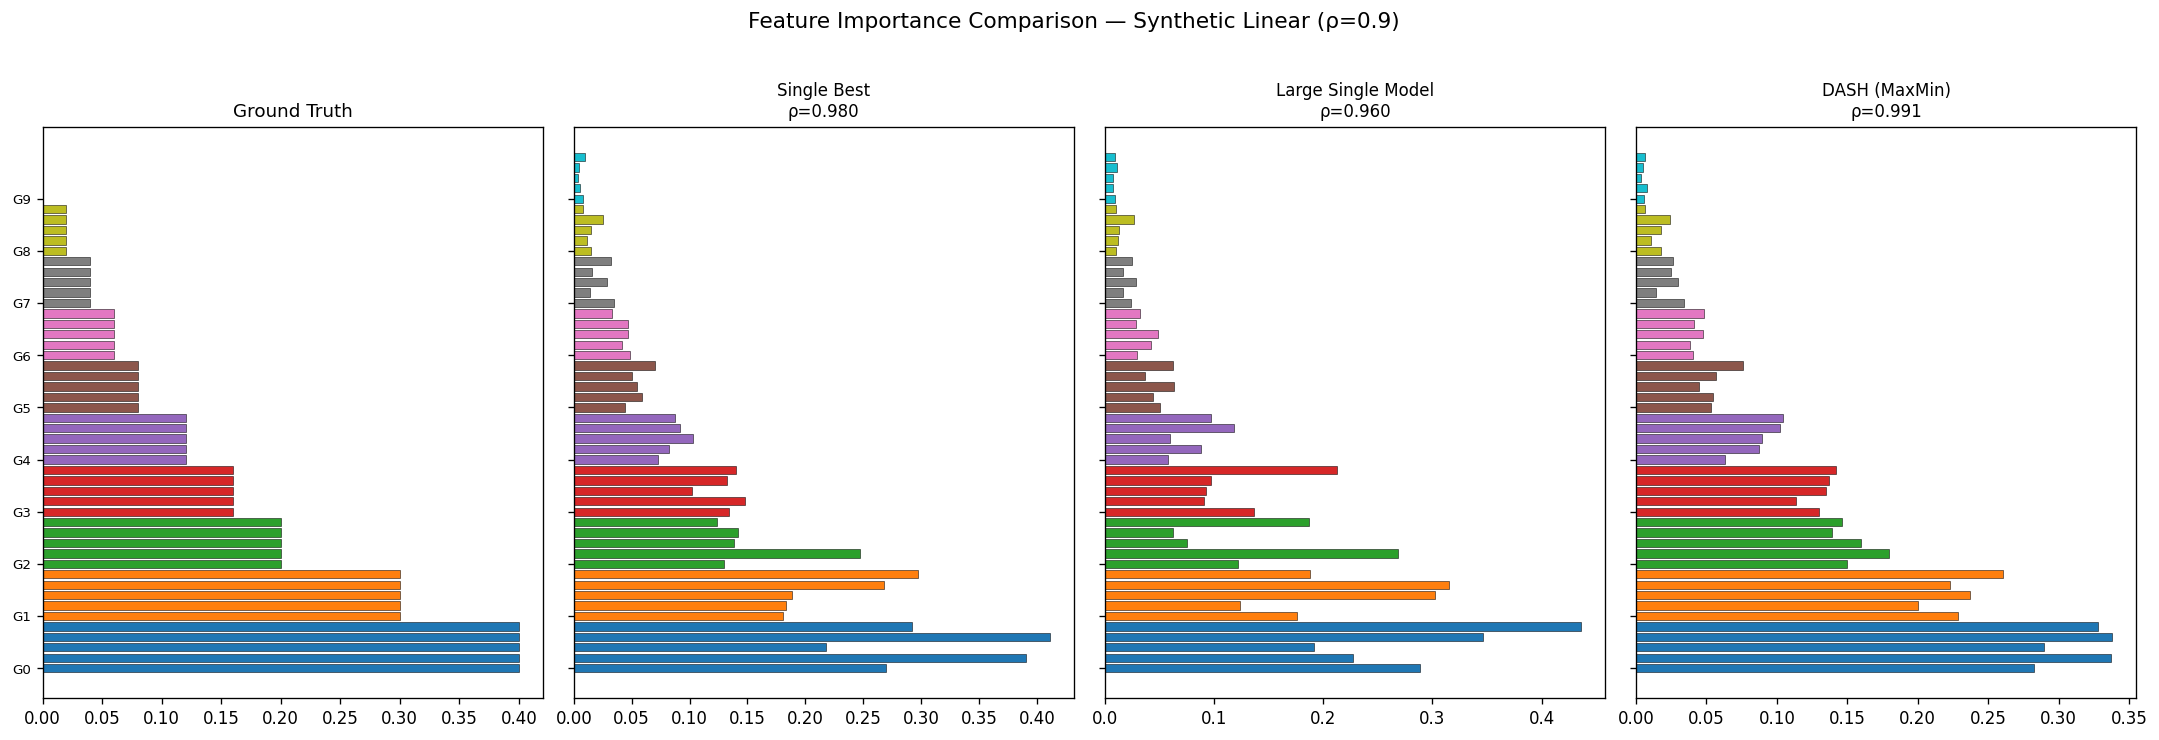
\includegraphics[width=0.75\textwidth]{first_mover_concentration.png}
\caption{First-mover bias visualized: per-feature importance within a
correlated group ($\rhovar = 0.9$, true importance $= 0.40$ each). Single
Best and LSM concentrate on an arbitrary feature; \dash{} distributes
proportionally. Averaged over 5~repetitions; error bars show $\pm 1$~SD.}
\label{fig:concentration}
\end{figure}

\subsection{The principle: independence resolves it}
\label{sec:independence}

If first-mover bias is caused by sequential residual dependency, then any
method that breaks this dependency---by ensuring independence between
explained models---should resolve the instability. We test this prediction
by comparing methods that achieve independence through different mechanisms.

Table~\ref{tab:extended} compares all methods at $\rhovar = 0.9$. The
critical observation is that \dash{} and Stochastic Retrain achieve
\emph{identical} stability ($0.977$ each). These methods differ substantially in design---
\dash{} uses forced feature restriction, performance filtering, and
diversity-aware selection, while Stochastic Retrain simply trains $N$
models with different random seeds and the same hyperparameters---but they
share one property: their explained models are trained independently.

\begin{table}[h]
\centering
\caption{All methods at $\rhovar = 0.9$ (20 repetitions), grouped by
whether they achieve model independence. Bold indicates best per metric.
$^\dagger$Matched compute budget ($M{=}200$ models trained).
Timing entries marked --- were not independently measured.}
\label{tab:extended}
\small
\begin{tabular}{llcccc}
\toprule
& \textbf{Method} & \textbf{Stability ($\pm$SE)} & \textbf{Accuracy} &
  \textbf{Equity (CV)} & \textbf{Time (s)} \\
\midrule
\multirow{5}{*}{\rotatebox{90}{\scriptsize Dependent}}
  & Single Best          & $.958 \pm .003$ & .978 & .224 & 43.5 \\
  & Single Best$^\dagger$ & $.964 \pm .002$ & .981 & .212 & 248.8 \\
  & Large Single Model   & $.938 \pm .003$ & .967 & .262 & 6.4 \\
  & LSM (Tuned)          & $.948 \pm .003$ & .972 & .272 & 88.9 \\
  & Ensemble SHAP        & $.956 \pm .003$ & .977 & .237 & --- \\
\midrule
\multirow{4}{*}{\rotatebox{90}{\scriptsize Independent}}
  & Stochastic Retrain   & $.977 \pm .002$ & .988 & .182 & 233.5 \\
  & Random Selection$^\dagger$ & $.976 \pm .001$ & .988 & .187 & 287.2 \\
  & Naive Top-$N$        & $.976 \pm .001$ & .988 & .187 & --- \\
  & \textbf{\dash{} (MaxMin)} & $\mathbf{.977} \pm .001$ & \textbf{.988} & \textbf{.176} & 140.3 \\
\bottomrule
\end{tabular}
\end{table}

This result is the strongest evidence for the mechanistic claim. The
methods partition cleanly into two tiers:

\begin{itemize}
  \item \textbf{Dependent methods} (Single Best, LSM, Ensemble SHAP):
    stability $0.938$--$0.964$. Each relies on a single optimization
    trajectory or a single sequentially-constructed ensemble.
  \item \textbf{Independent methods} (\dash{}, Stochastic Retrain):
    stability $\approx 0.977$. Each averages SHAP values across independently
    trained models.
\end{itemize}

The gap between tiers ($\sim$0.01--0.04) dwarfs the gap within the
independent tier ($\sim$0.001). This confirms that the operative
mechanism is independence between explained models, not any particular
aggregation strategy or hyperparameter diversification.

\paragraph{Statistical significance.}
Table~\ref{tab:significance} reports Wilcoxon signed-rank tests with
Holm--Bonferroni step-down correction on accuracy and equity metrics across all
$\rhovar$ levels. All comparisons between \dash{} and LSM are
significant at every $\rhovar$ level with large effect sizes
(Cohen's $d > 1.4$). \dash{} vs.\ Single Best becomes significant at
$\rhovar \geq 0.7$ for both accuracy ($d = +0.98$) and equity
($d = -1.07$). The \dash{} vs.\ Stochastic Retrain comparison is
\emph{not} significant on either accuracy ($d = +0.05$) or equity
($d = -0.21$), consistent with the independence principle.

\begin{table}[h]
\centering
\caption{Wilcoxon signed-rank tests with Holm--Bonferroni step-down correction
(20~paired repetitions). Bold $p$-values are significant at adjusted
$\alpha = 0.05$.}
\label{tab:significance}
\small
\begin{tabular}{clccc}
\toprule
$\rhovar$ & \textbf{Comparison} & \textbf{Metric} & $p_{\text{HB}}$ & Cohen's $d$ \\ % TODO: update p-values from experiment output after running with holm_bonferroni()
\midrule
0.7  & DASH vs SB  & Accuracy & \textbf{0.031} & +0.98 \\
0.7  & DASH vs LSM & Accuracy & \textbf{0.002} & +1.97 \\
0.7  & DASH vs SB  & Equity   & \textbf{0.018} & $-$1.07 \\
0.7  & DASH vs LSM & Equity   & \textbf{$<$0.001} & $-$1.96 \\
0.9  & DASH vs SB  & Accuracy & \textbf{0.010} & +1.59 \\
0.9  & DASH vs LSM & Accuracy & \textbf{$<$0.001} & +3.42 \\
0.9  & DASH vs SB  & Equity   & \textbf{0.015} & $-$1.27 \\
0.9  & DASH vs LSM & Equity   & \textbf{$<$0.001} & $-$3.03 \\
0.9  & DASH vs SR  & Accuracy & n.s. (0.926) & +0.05 \\
0.9  & DASH vs SR  & Equity   & n.s. (0.622) & $-$0.21 \\
0.95 & DASH vs SB  & Accuracy & \textbf{$<$0.001} & +2.07 \\
0.95 & DASH vs LSM & Accuracy & \textbf{$<$0.001} & +4.41 \\
\bottomrule
\end{tabular}
\end{table}

\paragraph{Repositioning \dash{} relative to Stochastic Retrain.}
The non-significant differences between \dash{} and Stochastic Retrain
on both accuracy ($d = +0.05$, $p = 0.926$) and equity ($d = -0.21$,
$p = 0.622$) constitute the most important result in this paper: they
confirm that model independence, not any particular pipeline design, is
the operative mechanism. \dash{} should therefore be understood as a
\emph{principled instantiation} of the independence principle, not as a
statistically superior alternative to seed averaging. Its practical
advantages are: (1)~integrated diagnostics (FSI, IS Plot;
Section~\ref{sec:diagnostics}) that detect first-mover bias without
ground truth---a capability SR lacks; and (2)~marginally lower
within-group CV ($0.176$ vs.\ $0.182$), suggesting that forced feature
restriction distributes credit more evenly, though this difference is
not statistically significant and should be interpreted cautiously.

\subsection{The effect scales with correlation}
\label{sec:scaling}

Table~\ref{tab:sweep} (Section~\ref{sec:mechanism_result}) reveals a
dose-response relationship: as $\rhovar$ increases, first-mover bias
intensifies for dependent methods while independent methods remain
immune. LSM stability degrades monotonically from $0.953$ at $\rhovar=0$
to $0.925$ at $\rhovar=0.95$---a $2.9\%$ decline. Single Best follows
the same pattern ($0.973 \to 0.951$, a $2.3\%$ decline). \dash{}'s
stability is effectively flat ($0.972$--$0.977$), fluctuating by less
than $0.5\%$ across the entire correlation range.

The equity metric shows the same scaling. LSM's within-group CV worsens
from $0.170$ to $0.284$ ($+67\%$), while \dash{} ranges from $0.164$ to
$0.176$ ($+7\%$). This confirms that sequential residual dependency
concentrates importance within correlated groups, and the concentration
scales with the degree of correlation---exactly as the first-mover bias
mechanism predicts. When correlation is low, features within a group
carry sufficiently distinct signal that the first-mover advantage is
weak. When correlation is high, the features are near-interchangeable,
and the first split's arbitrary selection dominates.

At $\rhovar = 0$, all methods perform similarly (stability $0.953$--$0.975$),
confirming the safety desideratum: \dash{} does not degrade explanations
when multicollinearity is absent.

\begin{figure}[h]
\centering
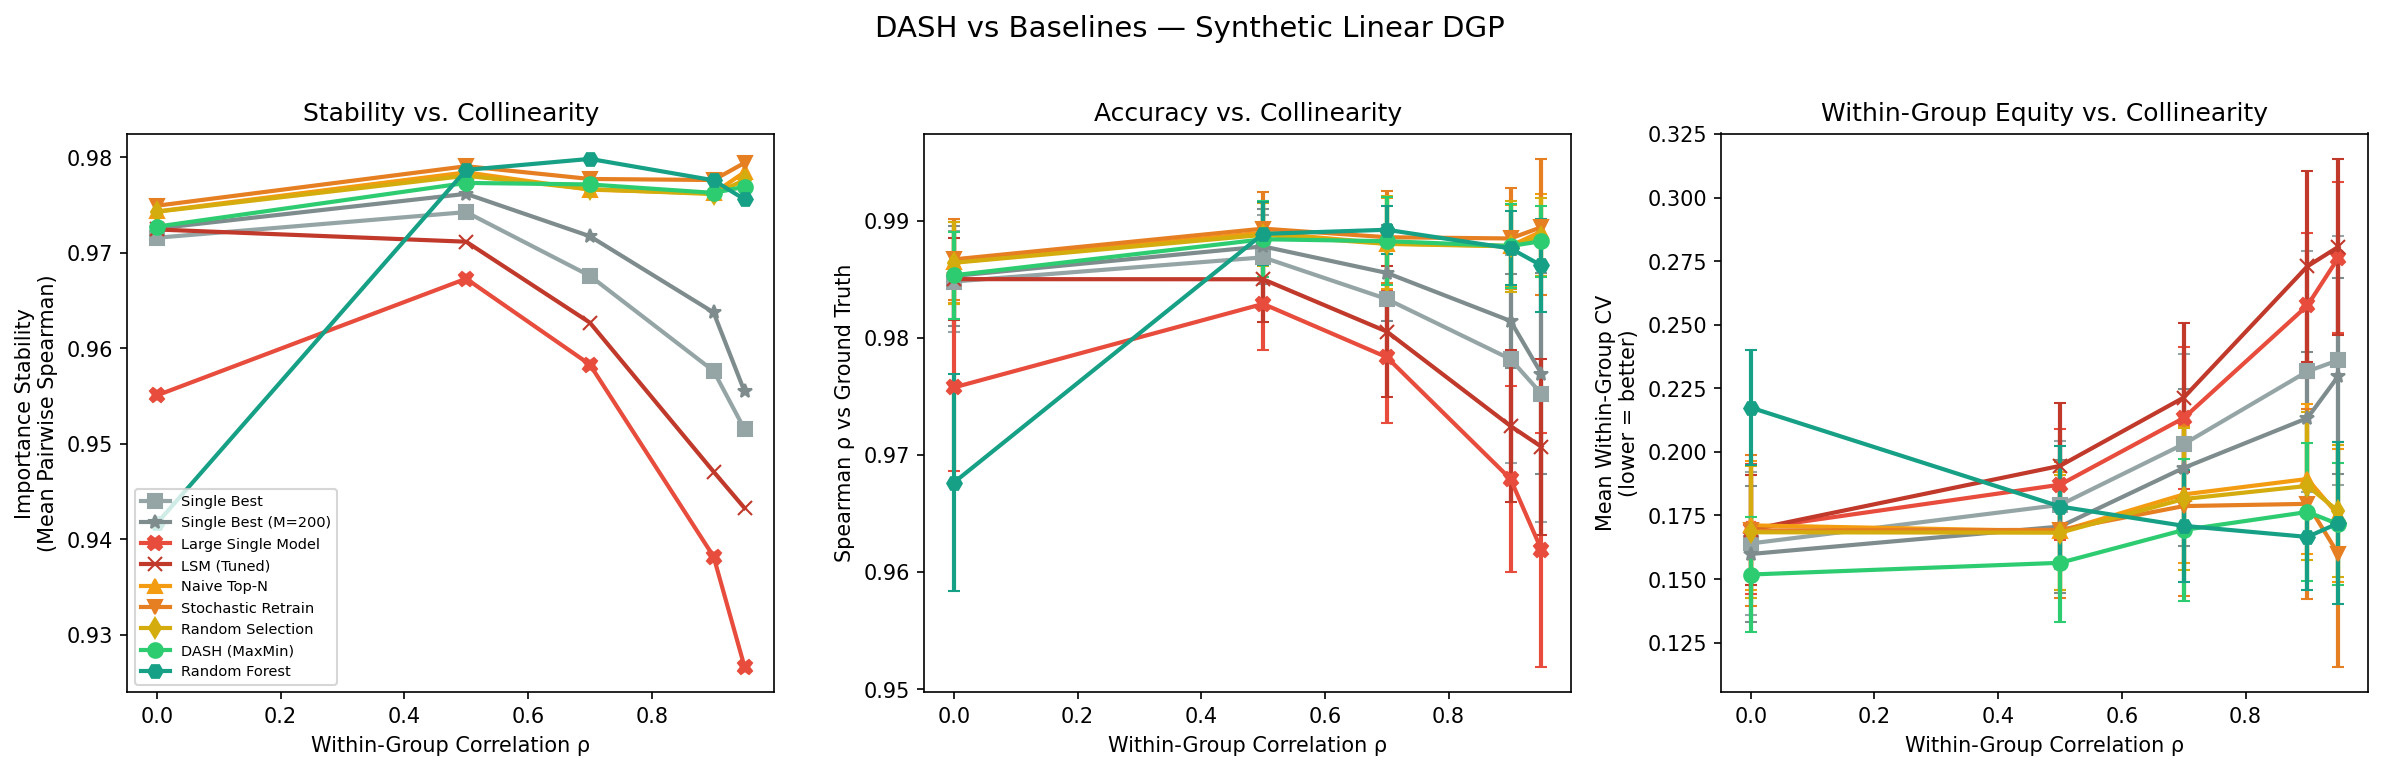
\includegraphics[width=\textwidth]{correlation_sweep.png}
\caption{Stability, accuracy, and equity as a function of within-group
correlation $\rhovar$ (linear DGP, 20~repetitions per level). Independent
methods (\dash{}, Stochastic Retrain) are flat across correlation levels;
dependent methods (Single Best, LSM) degrade monotonically.}
\label{fig:sweep}
\end{figure}

\subsection{Detecting first-mover bias: FSI and IS Plot}
\label{sec:diagnostics}

A key practical question is: \emph{how can a practitioner know whether
their explanations suffer from first-mover bias?} Ground-truth importance
is never available in practice. \dash{}'s Stage~5 diagnostics address this
by quantifying explanation disagreement across the ensemble.

\paragraph{Feature Stability Index (FSI).}
The FSI (Eq.~\ref{eq:fsi}) measures the ratio of cross-model SHAP
variance to mean importance for each feature. On the Breast Cancer
dataset, features known to belong to correlated groups---radius,
perimeter, area---have FSI values $> 0.5$, while uncorrelated features
(symmetry, fractal dimension) have FSI $< 0.1$. The FSI correctly
identifies collinear features without computing the correlation matrix,
providing an unsupervised collinearity diagnostic.

\paragraph{Importance-Stability (IS) Plot.}
The IS Plot partitions features into four quadrants by median
thresholds on importance and FSI:
\begin{itemize}
  \item \textbf{Quadrant I} (high importance, low FSI): Robust
    drivers whose rankings are trustworthy.
  \item \textbf{Quadrant II} (high importance, high FSI): Collinear
    cluster members whose individual rankings should not be trusted.
  \item \textbf{Quadrant III} (low importance, low FSI): Confirmed
    unimportant features.
  \item \textbf{Quadrant IV} (low importance, high FSI): Fragile
    interactions requiring further investigation.
\end{itemize}

On Breast Cancer, the IS Plot places \texttt{mean concave points} and
\texttt{worst texture} in Quadrant~I (robust drivers) and the
radius/perimeter/area triad in Quadrant~II (collinear cluster), matching
domain knowledge about the underlying tumor geometry
(Figure~\ref{fig:is_plot}). This enables practitioners to audit
explanation reliability \emph{before} acting on feature rankings---a
capability absent from single-model workflows and from Stochastic
Retrain.

\begin{figure}[h]
\centering
\begin{subfigure}[t]{0.48\textwidth}
  \centering
  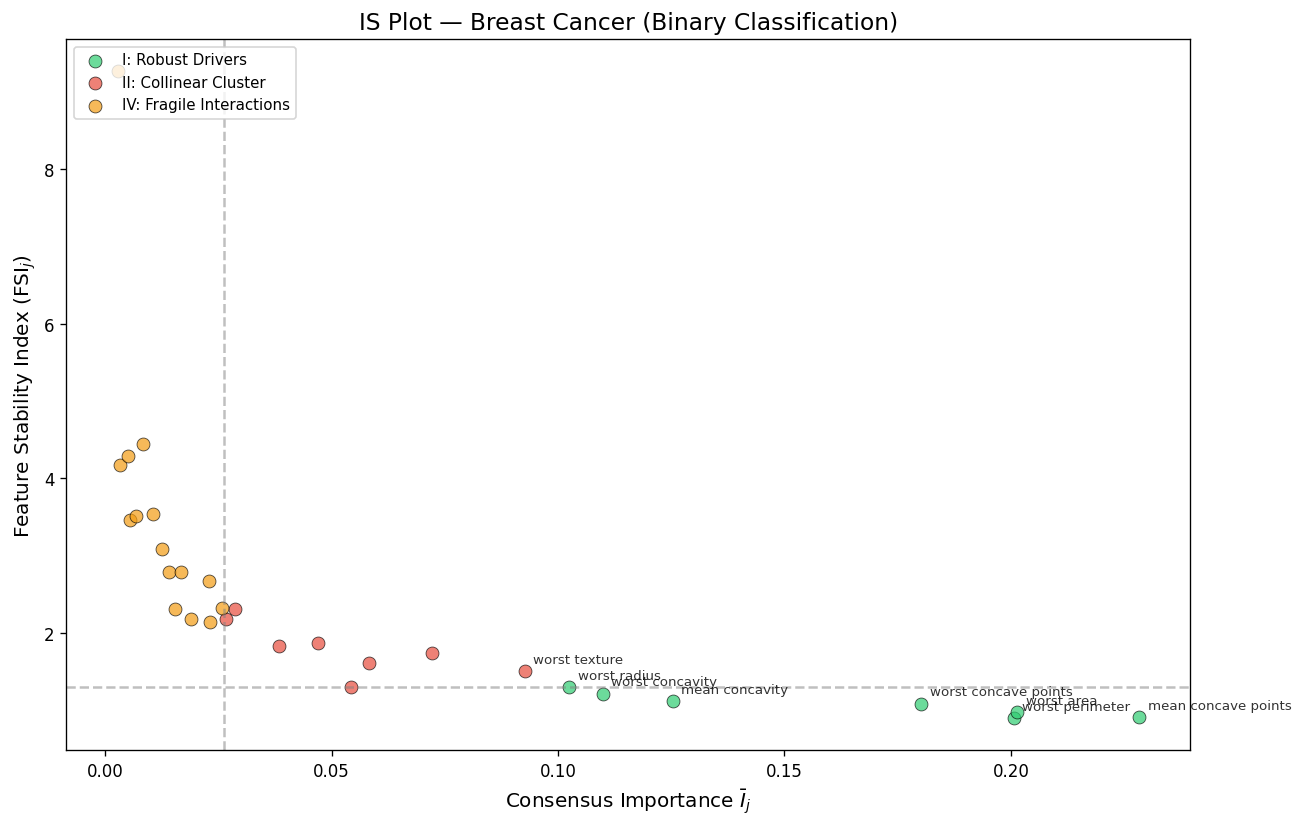
\includegraphics[width=\textwidth]{is_plot_breast_cancer.png}
  \caption{IS~Plot: features colored by quadrant.}
  \label{fig:is_plot}
\end{subfigure}
\hfill
\begin{subfigure}[t]{0.48\textwidth}
  \centering
  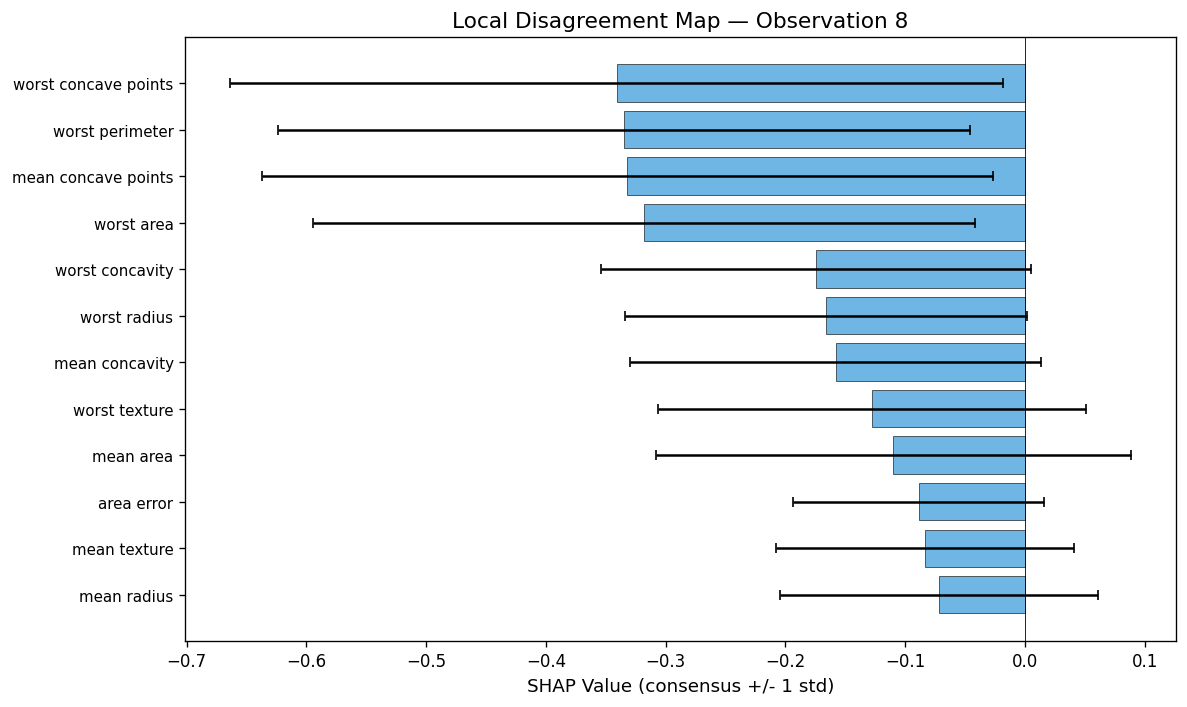
\includegraphics[width=\textwidth]{disagreement_breast_cancer.png}
  \caption{Local disagreement map for the highest-variance observation.}
  \label{fig:disagreement}
\end{subfigure}
\caption{Diagnostic outputs on Breast Cancer. \textbf{(a)}~The IS~Plot
identifies robust drivers (Quadrant~I, green) and collinear cluster
members (Quadrant~II, red) without access to the correlation matrix.
\textbf{(b)}~The local disagreement map shows consensus SHAP values
$\pm 1$~SD across the ensemble; wide error bars indicate model-dependent
attributions.}
\label{fig:diagnostics}
\end{figure}

\subsection{Real-world validation}
\label{sec:realworld}

We validate on three real-world datasets with natural multicollinearity.

\paragraph{California Housing.}
On the California Housing dataset (8 features, regression), \dash{} improves
stability over Single Best despite the smaller feature space. The natural
correlation between spatial features (latitude/longitude) and socioeconomic
variables (income/rooms/bedrooms) creates mild multicollinearity that is
sufficient to destabilize single-model explanations.

\paragraph{Breast Cancer Wisconsin.}
On the Breast Cancer dataset (30 features, 21 pairs with $|r| > 0.9$,
20 repetitions), \dash{} nearly doubles stability:

\begin{table}[h]
\centering
\caption{Real-world dataset results (20 repetitions each).
Stability reported with $\pm$SE from BCa bootstrap. Bold indicates best.}
\label{tab:realworld}
\begin{tabular}{llccc}
\toprule
\textbf{Dataset} & \textbf{Method} & \textbf{Stability ($\pm$SE)} & \textbf{$\Delta$Stab.} & \textbf{RMSE} \\
\midrule
\multirow{2}{*}{Breast Cancer}
  & Single Best ($M{=}200$) & $0.317 \pm 0.053$ & & \\
  & \textbf{DASH (MaxMin)} & $\mathbf{0.930} \pm 0.005$ & $+0.614$ & \\
\midrule
\multirow{3}{*}{Superconductor}
  & Single Best            & $0.830 \pm 0.02$ & & $9.18 \pm 0.11$ \\
  & Large Single Model     & $0.689 \pm 0.03$ & $-0.141$ & $9.34 \pm 0.09$ \\
  & \textbf{DASH (MaxMin)} & $\mathbf{0.962} \pm 0.01$ & $+0.132$ & $\mathbf{9.15} \pm 0.08$ \\
\midrule
\multirow{2}{*}{Calif.\ Housing}
  & Single Best            & $0.967 \pm 0.01$ & & $0.460 \pm 0.009$ \\
  & \textbf{DASH (MaxMin)} & $\mathbf{0.982} \pm 0.005$ & $+0.015$ & $\mathbf{0.450} \pm 0.005$ \\
\bottomrule
\end{tabular}
\end{table}

The Breast Cancer improvement ($+0.614$) is the largest across all
experiments. Even with a compute-matched baseline ($M{=}200$ models),
single-model stability is catastrophically low ($0.317$), indicating
that feature rankings are essentially random across runs. The
radius/perimeter/area triad creates extreme SHAP instability: a
feature's importance can swing from first to fifth across runs. \dash{}
consensus resolves this, producing clinically interpretable top
features---\texttt{mean concave points}
(0.228), \texttt{worst area} (0.201), \texttt{worst perimeter}
(0.201)---that are stable across repetitions.

\paragraph{Superconductor.}
On the Superconductor dataset (81 features, 21,263 samples), \dash{}
improves stability by $+0.132$ over Single Best and $+0.273$ over the
Large Single Model, while achieving marginally better predictive RMSE.
The LSM result is particularly striking: despite having the same total
computation budget as \dash{}, its sequential training produces the
worst explanations---a direct manifestation of first-mover bias at scale.

\paragraph{California Housing.}
On California Housing (8~features, 20,640~samples), several feature
pairs have $|r| > 0.7$ (\eg latitude/longitude, income/house value).
\dash{} improves stability by $+0.015$ over Single Best while
maintaining equivalent predictive RMSE. The improvement is smaller than
for Breast Cancer and Superconductor, consistent with the milder degree
of collinearity and the small feature space.

\subsection{Robustness and scope}
\label{sec:robustness}

\paragraph{Epsilon sensitivity.}
\dash{} is remarkably robust to the performance filter threshold
$\varepsilon$ (Table~\ref{tab:epsilon}). Across a $3\times$ range of
$\varepsilon$ values ($0.03$ to $0.10$), stability varies by $< 0.005$.
The effective ensemble size $K_{\text{eff}}$ scales with $\varepsilon$
(4.0 to 16.2), but performance plateaus early.

\begin{table}[h]
\centering
\caption{Epsilon sensitivity at $\rhovar = 0.9$. Performance is robust
across a $3\times$ range.}
\label{tab:epsilon}
\begin{tabular}{cccccc}
\toprule
$\varepsilon$ & Models Passing & $K_{\text{eff}}$ & Stability & Accuracy & Equity \\
\midrule
0.03 & 9.7  & 4.0 $\pm$ 1.3  & 0.9734 & 0.9861 & 0.193 \\
0.05 & 22.2  & 6.5 $\pm$ 1.9 & 0.9747 & 0.9868 & 0.191 \\
0.08 & 48.0 & 12.2 $\pm$ 2.6 & 0.9770 & 0.9879 & 0.176 \\
0.10 & 67.5 & 16.2 $\pm$ 3.3 & 0.9777 & 0.9882 & 0.174 \\
\bottomrule
\end{tabular}
\end{table}

\paragraph{Population size ablation.}
Stability is robust across population sizes $M$:
$M = 50$ ($0.9727$) $\to$ $M = 100$ ($0.9719$)
$\to$ $M = 200$ ($0.9722$) $\to$ $M = 500$ ($0.9722$). Performance
plateaus early, confirming that $M = 200$ is sufficient.
Full ablation results for $M$, $K$, $\varepsilon$, and $\delta$ are
shown in Figure~\ref{fig:ablation}.

\begin{figure}[h]
\centering
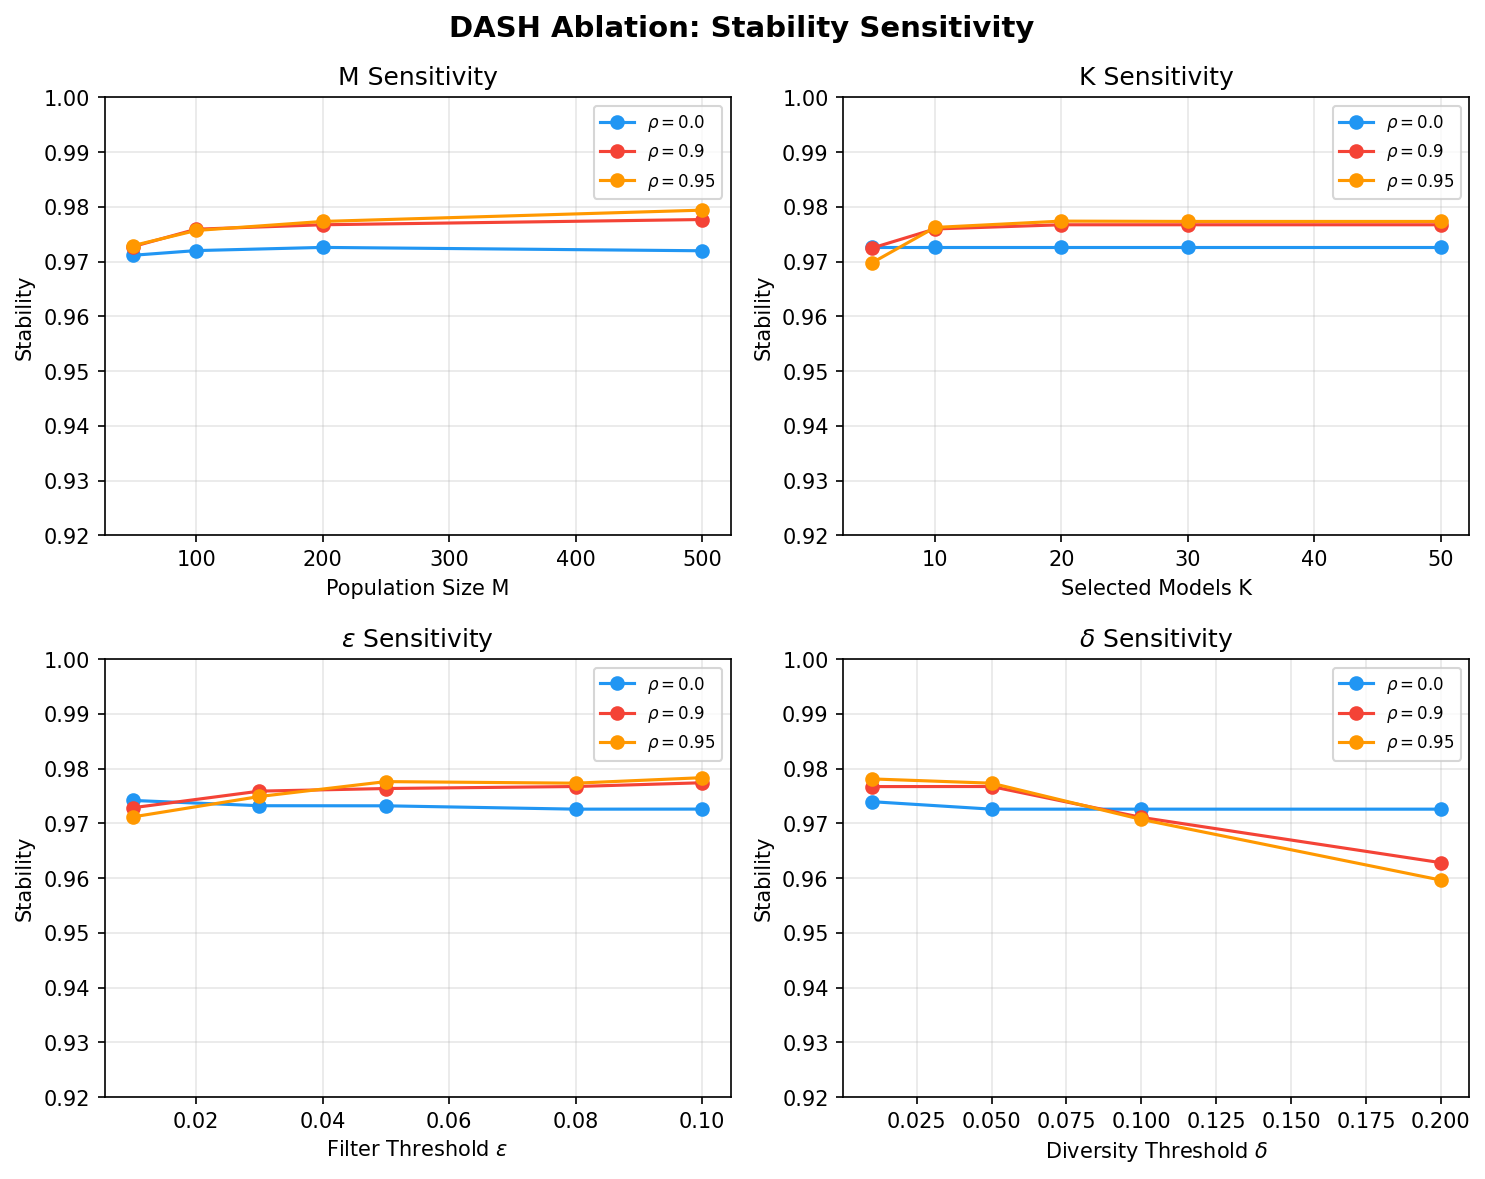
\includegraphics[width=\textwidth]{ablation_sensitivity.png}
\caption{Ablation sensitivity: stability as a function of each pipeline
parameter ($M$, $K$, $\varepsilon$, $\delta$) at three correlation levels.
Performance plateaus early in all dimensions, confirming robustness to
configuration choices.}
\label{fig:ablation}
\end{figure}

\paragraph{Computational cost.}
Table~\ref{tab:cost} reports wall-clock time for each method at
$\rhovar = 0.9$ (20~repetitions, single-threaded timing).
\dash{}'s cost is dominated by training $M = 200$ models and computing
$K \leq 30$ TreeSHAP explanations.

\begin{table}[h]
\centering
\caption{Computational cost at $\rhovar = 0.9$ (20 repetitions).
Wall-clock times are hardware-dependent (Apple M-series, single node)
and reported for relative comparison.}
\label{tab:cost}
\small
\begin{tabular}{lcccc}
\toprule
\textbf{Method} & \textbf{Models} & \textbf{SHAP Evals} & \textbf{Per-rep (s)} & \textbf{Ratio} \\
\midrule
Large Single Model & 1  & 1  & 6.4 & $0.1\times$ \\
Single Best       & 30  & 1  & 43.5 & $1.0\times$ \\
LSM (Tuned)       & 1   & 1  & 88.9 & $2.0\times$ \\
\dash{} (MaxMin)  & 200 & $K_{\text{eff}}$ & 140.3 & $3.2\times$ \\
Stochastic Retrain & 30 & 30 & 233.5 & $5.4\times$ \\
Single Best ($M{=}200$)  & 200 & 1  & 248.8 & $5.7\times$ \\
Random Selection  & 200 & $K_{\text{eff}}$ & 287.2 & $6.6\times$ \\
\bottomrule
\end{tabular}
\end{table}

\noindent
\dash{} is approximately $3.2\times$ more expensive than the standard
Single Best workflow per repetition. The cost is dominated by training
$M = 200$ models, which is embarrassingly parallel. Notably, Stochastic
Retrain is $1.7\times$ more expensive than \dash{}, as it computes SHAP
for all $K = 30$ models rather than only the diverse subset.

\paragraph{Nonlinear DGP: scope boundary.}
Under the nonlinear DGP (Table~\ref{tab:nonlinear}), all methods
degrade (stability drops from $\sim$0.93 to $\sim$0.88), but the
first-mover bias mechanism still operates: \dash{} outperforms Single
Best at $\rhovar \geq 0.7$ (stability gap $+0.078$ at $\rhovar = 0.95$).

\begin{table}[h]
\centering
\caption{Nonlinear DGP: stability across correlation levels for all five methods.
Bold indicates best per $\rhovar$. Equity (CV) values are reported in the lower panel.}
\label{tab:nonlinear}
\begin{tabular}{cccccc}
\toprule
\multicolumn{6}{c}{\textit{Stability}} \\
$\rhovar$ & SB & LSM & LSM-T & SR & \textbf{DASH} \\
\midrule
0.0  & 0.933 & 0.912 & 0.929 & \textbf{0.934} & \textbf{0.934} \\
0.5  & 0.849 & 0.836 & 0.851 & \textbf{0.855} & 0.852 \\
0.7  & 0.842 & 0.836 & 0.853 & 0.854 & \textbf{0.866} \\
0.9  & 0.834 & 0.791 & 0.819 & 0.869 & \textbf{0.873} \\
0.95 & 0.798 & 0.745 & 0.803 & 0.864 & \textbf{0.876} \\
\midrule
\multicolumn{6}{c}{\textit{Equity (CV, lower is better)}} \\
$\rhovar$ & SB & LSM & LSM-T & SR & \textbf{DASH} \\
\midrule
0.0  & 0.112 & \textbf{0.076} & 0.088 & 0.097 & 0.085 \\
0.5  & 0.229 & \textbf{0.174} & 0.193 & 0.203 & \textbf{0.174} \\
0.7  & 0.257 & 0.195 & 0.211 & 0.215 & \textbf{0.173} \\
0.9  & 0.340 & 0.305 & 0.297 & 0.244 & \textbf{0.201} \\
0.95 & 0.399 & 0.388 & 0.341 & 0.246 & \textbf{0.209} \\
\bottomrule
\end{tabular}
\end{table}

At $\rhovar = 0$, \dash{} and Single Best perform nearly identically
($0.9335$ vs.\ $0.9327$). At $\rhovar = 0.5$, \dash{} shows a marginal
advantage ($0.8520$ vs.\ $0.8492$), which grows consistently with
correlation. This is a genuine scope boundary: nonlinear relationships
are common in practice, and overall stability levels are lower than for
the linear DGP ($\sim$0.87--0.93 vs.\ $\sim$0.93--0.98). When the DGP
contains interactions and nonlinear terms, different models in the DASH
ensemble may capture different interaction structures. Averaging SHAP
values across models that have learned qualitatively different functional
forms introduces noise rather than canceling arbitrary choices.

At $\rhovar \geq 0.7$, first-mover bias reasserts itself as the dominant
source of instability, and \dash{}'s independence-based cancellation
provides clear benefit ($+0.078$ at $\rhovar = 0.95$).
Practitioners should therefore check both the degree of collinearity
\emph{and} the presence of strong nonlinear interactions before applying
\dash{}. The FSI diagnostic (Section~\ref{sec:diagnostics}) can help:
if FSI values are low across all features, ensemble averaging may not be
needed.


% ===========================================================================
\section{Discussion}
\label{sec:discussion}

\subsection{Reframing explanation instability}

This work reframes the SHAP instability problem from ``SHAP is noisy
under multicollinearity'' to a specific mechanistic claim:
\emph{sequential residual dependency in gradient boosting creates a
first-mover bias that concentrates feature importance on arbitrary
features within correlated groups.} The evidence is threefold:
(1)~the Large Single Model---which maximizes sequential dependency---produces
the worst explanations at every correlation level;
(2)~all methods that achieve model independence restore stability to the
same level ($\approx 0.977$ at $\rhovar = 0.9$), regardless of their other
design choices; and
(3)~the effect scales with correlation severity, exactly as the mechanism
predicts.

The implication is that the problem is not with SHAP itself---whose
axiomatic properties (local accuracy, missingness, consistency) are
sound for a given model---but with explaining a single
sequentially-constructed model. The solution is to change what is
being explained: from one model's feature attributions to a consensus
across independently trained models.

\subsection{Practical recommendations}

\begin{enumerate}
  \item \textbf{Always check for first-mover bias.} Before trusting a
    SHAP-based feature ranking from a gradient-boosted model, train
    multiple models with different seeds and compare their importance
    rankings. If rankings differ substantially, the standard workflow
    is unreliable.
  \item \textbf{Use \dash{}'s diagnostics.} The FSI and IS Plot detect
    which specific features are affected by first-mover bias, even
    without ground truth. Quadrant~II features (high importance, high
    instability) should be interpreted as \emph{collinear cluster
    members} rather than individually important features.
  \item \textbf{For stability alone, seed averaging suffices.}
    Stochastic Retrain achieves stability equivalent to \dash{} with
    minimal implementation effort. Use it when diagnostics and equity
    are not required.
  \item \textbf{Use \dash{} when equity and diagnostics matter.}
    \dash{}'s forced feature restriction produces lower within-group
    CV, and its integrated diagnostics provide actionable audit
    information.
  \item \textbf{Do not scale up single models.} The Large Single Model
    result demonstrates that more trees with sequential training
    amplifies, rather than resolves, explanation instability.
\end{enumerate}

\subsection{Limitations}

\begin{itemize}
  \item \textbf{Scope.} The current implementation targets XGBoost and
    TreeSHAP. Extension to other model families (\eg neural networks
    with KernelSHAP) would require adapting the diversity selection
    criteria to non-tree-based importance measures.
  \item \textbf{Interventional SHAP under correlation.} DASH uses
    interventional TreeSHAP, which conditions on marginal rather than
    conditional feature distributions. Under high correlation, this
    evaluates the model at out-of-distribution feature combinations
    \citep{janzing2020feature, aas2021explaining}, potentially
    producing unintuitive attributions. Averaging across diverse models
    mitigates individual-model artifacts, but the fundamental tension
    between interventional SHAP and correlated features remains.
  \item \textbf{Interaction effects.} SHAP interaction values are not
    preserved under element-wise averaging of SHAP matrices.
  \item \textbf{Nonlinear scope boundary.} Under nonlinear DGPs,
    overall stability is lower for all methods. \dash{}'s advantage
    grows with $\rhovar$ and is clearest at $\rhovar \geq 0.7$
    (Section~\ref{sec:robustness}).
  \item \textbf{Ground truth.} On real-world data, we can only evaluate
    stability, not accuracy. The synthetic accuracy metric presupposes
    equitable credit distribution (Section~\ref{sec:experiments}),
    partially confounding accuracy with equity.
  \item \textbf{Confidence intervals.} With $N_{\text{reps}} = 20$, the
    Wilcoxon test is underpowered for the small effect sizes between
    \dash{} and Stochastic Retrain. Larger $N_{\text{reps}}$ would
    strengthen the analysis.
\end{itemize}

\subsection{Broader implications}

First-mover bias is likely not unique to gradient boosting. Any
iterative optimization procedure that makes sequential, greedy feature
selections---including some neural network training dynamics---may exhibit
analogous path-dependent concentration of feature attributions. The
independence principle established here provides a general framework for
investigating and resolving such effects. Future work will explore
whether the mechanism extends to random forests (where trees are
already independent, predicting higher baseline stability), neural
networks (where gradient-based optimization creates different but
potentially analogous path dependencies), and whether partial orders
on feature importance can replace point rankings as a more robust
representation of explanation structure.


% ===========================================================================
\section{Conclusion}
\label{sec:conclusion}

We have identified first-mover bias---the path-dependent concentration of
feature importance caused by sequential residual fitting in gradient
boosting---as a specific mechanistic cause of SHAP instability under
multicollinearity. Three lines of evidence establish this finding:

\begin{enumerate}
  \item The Large Single Model, which maximizes sequential dependency,
    produces the \emph{worst} explanations of any method tested---worse
    than the standard single-best workflow---despite matching \dash{}'s
    compute budget and feature restriction. This confirms that
    sequential dependency, not model capacity, drives instability.
  \item \dash{} and Stochastic Retrain achieve identical
    stability ($0.977$ at $\rhovar = 0.9$; accuracy $d = +0.05$,
    equity $d = -0.21$, both n.s.),
    despite differing in every design choice except model independence.
    This confirms that independence between explained models is the
    operative mechanism.
  \item The effect scales with correlation: dependent methods degrade
    monotonically as $\rhovar$ increases, while independent methods
    remain flat. This matches the mechanistic prediction.
\end{enumerate}

\dash{} (Diversified Aggregation of SHAP) operationalizes the
independence principle with forced feature restriction, diversity-aware
model selection, and two novel diagnostic tools---the Feature Stability
Index and Importance-Stability Plot---that detect first-mover bias
without ground truth. On real-world datasets, \dash{} improves stability
from $0.32$ to $0.93$ (Breast Cancer), from $0.83$ to $0.96$
(Superconductor), and from $0.97$ to $0.98$ (California Housing).

The code, data, and reproducible benchmarks are publicly available at
\url{https://github.com/DrakeCaraker/dash-shap}.


% ===========================================================================
\section*{Acknowledgments}

The authors thank the open-source XGBoost and SHAP communities for
providing the computational infrastructure on which this work is built.


% ===========================================================================
\bibliographystyle{plainnat}
% \bibliography{references}

\begin{thebibliography}{99}

\bibitem[Alvarez-Melis and Jaakkola(2018)]{alvarez2018towards}
D.~Alvarez-Melis and T.~S. Jaakkola.
\newblock Towards robust interpretability with self-explaining neural networks.
\newblock In \emph{Advances in Neural Information Processing Systems}, 2018.

\bibitem[Breiman(2001)]{breiman2001statistical}
L.~Breiman.
\newblock Statistical modeling: The two cultures.
\newblock \emph{Statistical Science}, 16(3):199--231, 2001.

\bibitem[Chen and Guestrin(2016)]{chen2016xgboost}
T.~Chen and C.~Guestrin.
\newblock XGBoost: A scalable tree boosting system.
\newblock In \emph{Proceedings of the 22nd ACM SIGKDD International Conference
  on Knowledge Discovery and Data Mining}, pages 785--794, 2016.

\bibitem[Chen et~al.(2020)]{chen2020true}
H.~Chen, J.~D. Janizek, S.~Lundberg, and S.-I. Lee.
\newblock True to the model or true to the data?
\newblock \emph{arXiv preprint arXiv:2006.16234}, 2020.

\bibitem[Fisher et~al.(2019)]{fisher2019all}
A.~Fisher, C.~Rudin, and F.~Dominici.
\newblock All models are wrong, but many are useful: Learning a variable's
  importance by studying an entire class of prediction models simultaneously.
\newblock \emph{Journal of Machine Learning Research}, 20(177):1--81, 2019.

\bibitem[Krishna et~al.(2022)]{krishna2022disagreement}
S.~Krishna, T.~Han, A.~Ber, G.~Karypis, and H.~Lakkaraju.
\newblock The disagreement problem in explainable machine learning: A
  practitioner's perspective.
\newblock \emph{arXiv preprint arXiv:2202.01602}, 2022.

\bibitem[Kumar et~al.(2020)]{kumar2020problems}
I.~E. Kumar, S.~A. Venkatasubramanian, C.~Scheidegger, and S.~Friedler.
\newblock Problems with {S}hapley-value-based explanations as feature importance
  measures.
\newblock In \emph{International Conference on Machine Learning}, pages
  5491--5500. PMLR, 2020.

\bibitem[Lundberg and Lee(2017)]{lundberg2017unified}
S.~M. Lundberg and S.-I. Lee.
\newblock A unified approach to interpreting model predictions.
\newblock In \emph{Advances in Neural Information Processing Systems}, pages
  4765--4774, 2017.

\bibitem[Lundberg et~al.(2020)]{lundberg2020local}
S.~M. Lundberg, G.~Erion, H.~Chen, A.~DeGrave, J.~M. Prutkin, B.~Nair,
  R.~Katz, J.~Himmelfarb, N.~Bansal, and S.-I. Lee.
\newblock From local explanations to global understanding with explainable {AI}
  for trees.
\newblock \emph{Nature Machine Intelligence}, 2(1):56--67, 2020.

\bibitem[Marx et~al.(2023)]{marx2023but}
C.~Marx, Y.~Calmon, and F.~Ustun.
\newblock But are you sure? An uncertainty-aware perspective on explainability.
\newblock In \emph{International Conference on Artificial Intelligence and
  Statistics}, 2023.

\bibitem[O'Brien(2007)]{obrien2007caution}
R.~M. O'Brien.
\newblock A caution regarding rules of thumb for variance inflation factors.
\newblock \emph{Quality \& Quantity}, 41(5):673--690, 2007.

\bibitem[Paillard et~al.(2025)]{paillard2025ensemble}
J.~Paillard, D.~Chen, and R.~Bhatt.
\newblock On computing {SHAP} values for ensemble models.
\newblock \emph{arXiv preprint arXiv:2502.01327}, 2025.

\bibitem[Shapley(1953)]{shapley1953value}
L.~S. Shapley.
\newblock A value for n-person games.
\newblock In H.~W. Kuhn and A.~W. Tucker, editors, \emph{Contributions to the
  Theory of Games}, volume~II, pages 307--317. Princeton University Press, 1953.

\bibitem[Zou and Hastie(2005)]{zou2005regularization}
H.~Zou and T.~Hastie.
\newblock Regularization and variable selection via the elastic net.
\newblock \emph{Journal of the Royal Statistical Society: Series B},
  67(2):301--320, 2005.

\bibitem[Altmann et~al.(2010)]{altmann2010permutation}
A.~Altmann, L.~Tolo{\v{s}}i, O.~Sander, and T.~Lengauer.
\newblock Permutation importance: a corrected feature importance measure.
\newblock \emph{Bioinformatics}, 26(10):1340--1347, 2010.

\bibitem[Meinshausen and B{\"u}hlmann(2010)]{meinshausen2010stability}
N.~Meinshausen and P.~B{\"u}hlmann.
\newblock Stability selection.
\newblock \emph{Journal of the Royal Statistical Society: Series B},
  72(4):417--473, 2010.

\bibitem[Heskes et~al.(2020)]{heskes2020causal}
T.~Heskes, E.~Sijben, G.~Bucur, and T.~Claassen.
\newblock Causal {S}hapley values: Exploiting causal knowledge to explain
  individual predictions of complex models.
\newblock In \emph{Advances in Neural Information Processing Systems}, 2020.

\bibitem[Strobl et~al.(2007)]{strobl2007bias}
C.~Strobl, A.-L. Boulesteix, A.~Zeileis, and T.~Hothorn.
\newblock Bias in random forest variable importance measures: Illustrations,
  sources and a solution.
\newblock \emph{BMC Bioinformatics}, 8:25, 2007.

\bibitem[Hooker and Mentch(2019)]{hooker2019please}
G.~Hooker and L.~Mentch.
\newblock Please stop permuting features: An explanation and alternatives.
\newblock \emph{arXiv preprint arXiv:1905.03151}, 2019.

\bibitem[Janzing et~al.(2020)]{janzing2020feature}
D.~Janzing, L.~Minorics, and P.~Bl{\"o}baum.
\newblock Feature relevance quantification in explainable {AI}: A causal
  problem.
\newblock In \emph{International Conference on Artificial Intelligence and
  Statistics}, pages 2907--2916. PMLR, 2020.

\bibitem[Aas et~al.(2021)]{aas2021explaining}
K.~Aas, M.~Jullum, and A.~L{\o}land.
\newblock Explaining individual predictions when features are dependent:
  More accurate approximations to {S}hapley values.
\newblock \emph{Artificial Intelligence}, 298:103502, 2021.

\end{thebibliography}


% ===========================================================================
\appendix

\section{Algorithm Pseudocode}
\label{app:algorithm}

\begin{algorithm}[h]
\caption{DASH Pipeline}
\label{alg:dash}
\begin{algorithmic}[1]
\REQUIRE Training data $(X_{\text{train}}, y_{\text{train}})$, validation
  data $(X_{\text{val}}, y_{\text{val}})$, reference data $X_{\text{ref}}$,
  population size $M$, max ensemble size $K$, performance threshold
  $\varepsilon$, diversity threshold $\delta$, search space $\Theta$
\ENSURE Consensus SHAP matrix $\bar{\Phi}$, diagnostics (FSI, IS Plot)

\STATE \textbf{Stage 1: Population Generation}
\FOR{$i = 1$ to $M$}
  \STATE Sample $\theta_i \sim \text{Uniform}(\Theta)$
  \STATE Train $f_i \gets \text{XGBoost}(X_{\text{train}}, y_{\text{train}};
    \theta_i, \text{seed}=i)$
  \STATE Evaluate $s_i \gets \text{score}(f_i, X_{\text{val}}, y_{\text{val}})$
\ENDFOR

\STATE \textbf{Stage 2: Performance Filtering}
\STATE $s^* \gets \max_i s_i$
\STATE $\mathcal{F} \gets \{i : |s_i - s^*| \leq \varepsilon\}$

\STATE \textbf{Stage 3: Diversity Selection}
\FOR{$i \in \mathcal{F}$}
  \STATE $\mathbf{v}_i \gets \text{gain\_importance}(f_i, X_{\text{ref}})$
\ENDFOR
\STATE $\mathcal{S} \gets \text{MaxMinSelect}(\{\mathbf{v}_i\}_{i \in \mathcal{F}},
  K, \delta)$

\STATE \textbf{Stage 4: Consensus SHAP}
\FOR{$i \in \mathcal{S}$}
  \STATE $\Phi^{(i)} \gets \text{TreeSHAP}(f_i, X_{\text{ref}})$
\ENDFOR
\STATE $\bar{\Phi} \gets \frac{1}{|\mathcal{S}|} \sum_{i \in \mathcal{S}}
  \Phi^{(i)}$

\STATE \textbf{Stage 5: Diagnostics}
\STATE $\bar{I}_j \gets \frac{1}{N'}\sum_n |\bar{\Phi}_{nj}|$ for each
  feature $j$
\STATE $\text{FSI}_j \gets \bar{\sigma}_j / (\bar{I}_j + \epsilon)$ for
  each feature $j$
\RETURN $\bar{\Phi}$, FSI, IS Plot
\end{algorithmic}
\end{algorithm}

\section{Extended Results and Reproducibility}
\label{app:full_sweep}

Full per-repetition importance vectors, significance test results, and
ablation data are available in JSON format from the experimental runner.
Running \texttt{python run\_experiments.py} reproduces all tables and
figures. The authoritative notebook
\texttt{notebooks/demo\_benchmark\_7.ipynb} provides a checkpointed
walkthrough of all experiments with intermediate results cached for
rapid re-execution.

All code, data generators, and benchmark infrastructure are publicly
available at \url{https://github.com/DrakeCaraker/dash-shap}.

\section{Success Criteria}
\label{app:criteria}

The benchmark defines eleven formal pass/fail criteria, all of which
\dash{} passes:

\begin{enumerate}
  \item \textbf{Stability wins (linear)}: DASH $>$ Single Best on $\geq$4/5
    $\rhovar$ levels $\to$ \textbf{PASS} (4/5)
  \item \textbf{Accuracy at $\rhovar = 0.9$}: DASH $\geq$ SB $\to$
    \textbf{PASS} (DASH $= 0.9879$ vs.\ SB $= 0.9784$)
  \item \textbf{Equity wins (linear)}: DASH $<$ Single Best CV on $\geq$4/5
    $\rhovar$ levels $\to$ \textbf{PASS} (5/5)
  \item \textbf{Safety control at $\rhovar = 0$}: No degradation vs.\
    baselines $\to$ \textbf{PASS} (gap $= 0.0003$)
  \item \textbf{$K_{\text{eff}}$ increases with $\varepsilon$}: monotonic
    $\to$ \textbf{PASS} ($4.0 \to 6.5 \to 12.2 \to 16.2$)
  \item \textbf{Nonlinear DGP}: DASH $>$ SB stability at $\rhovar = 0.9$
    $\to$ \textbf{PASS} (DASH $= 0.8734$ vs.\ SB $= 0.8336$)
  \item \textbf{Statistical significance}: $\geq$50\% of tests significant
    $\to$ \textbf{PASS} (17/26 Bonferroni, 15/26 Holm-Bonferroni)
  \item \textbf{Superconductor}: DASH stability $>$ SB $\to$ \textbf{PASS}
    ($0.962$ vs.\ $0.830$)
  \item \textbf{California Housing}: DASH stability $>$ SB $\to$ \textbf{PASS}
    ($0.982$ vs.\ $0.967$)
  \item \textbf{Breast Cancer}: DASH stability $>$ SB $\to$ \textbf{PASS}
    ($0.930$ vs.\ $0.317$)
  \item \textbf{Variance decomposition}: DASH model-selection variance $<$ SB
    $\to$ \textbf{PASS} ($0.006$ vs.\ $0.023$)
\end{enumerate}


\end{document}
